\documentclass[tikz,border=10pt]{standalone}
\usepackage{tikz}
\usepackage{amsmath}
\usetikzlibrary{shapes.geometric, arrows.meta, positioning, fit, backgrounds, decorations.pathreplacing}

\begin{document}
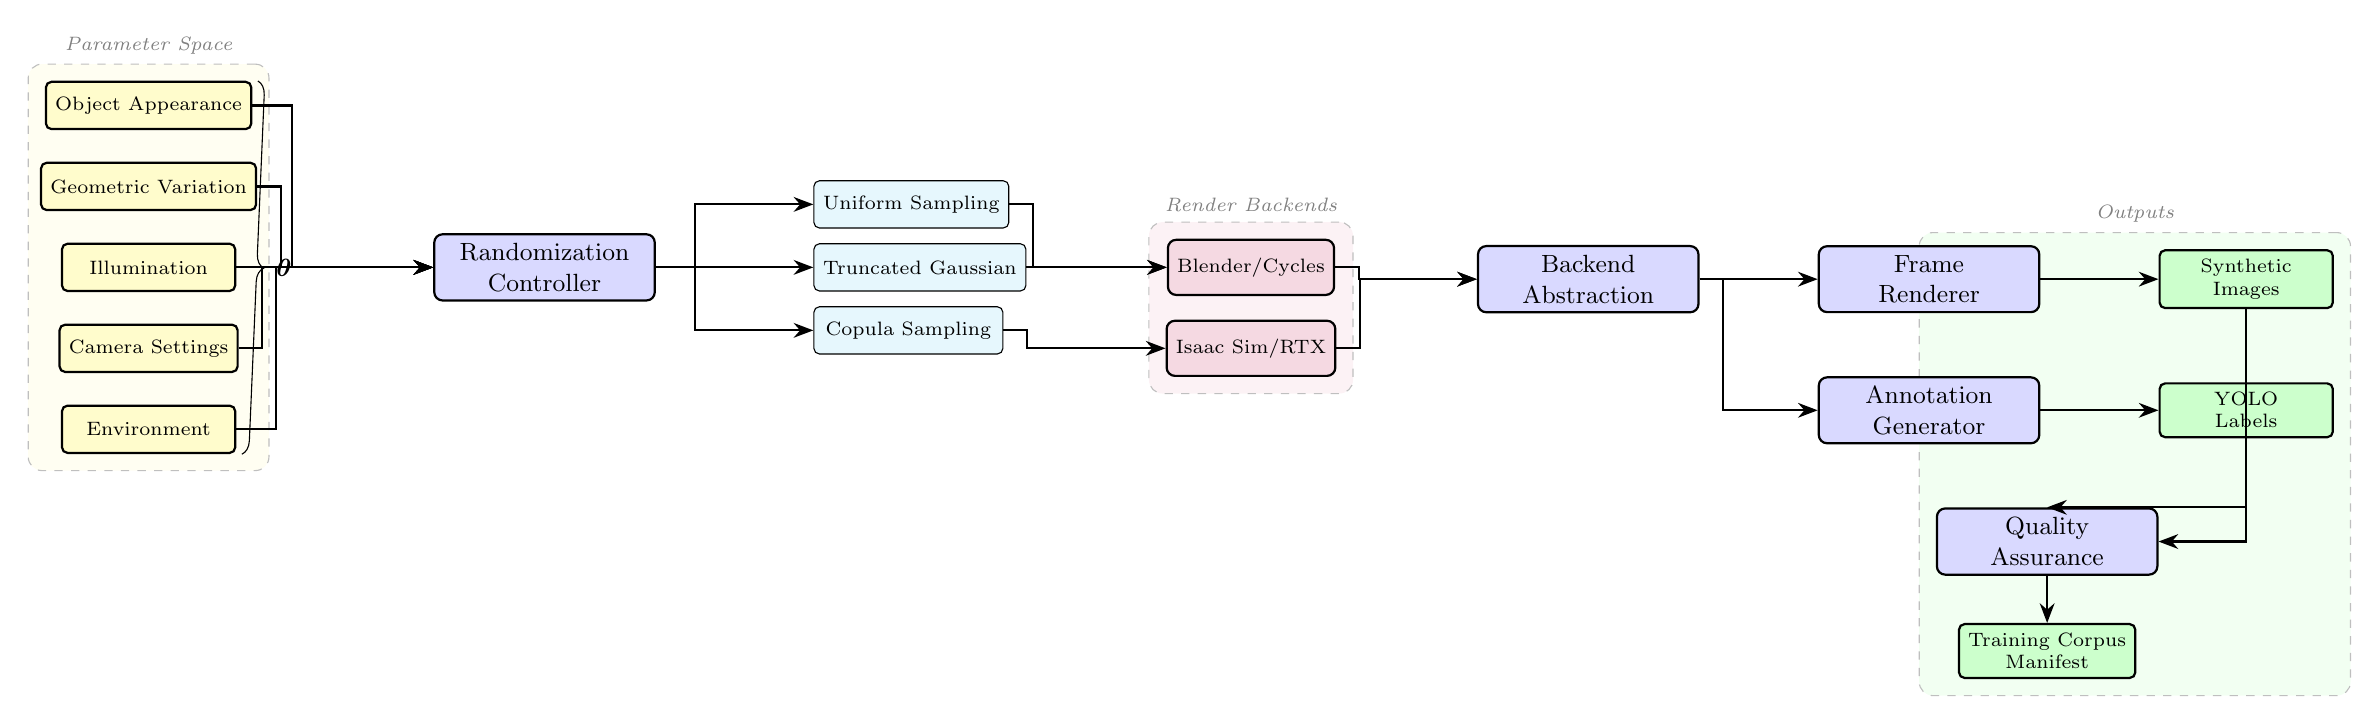
\begin{tikzpicture}[
    node distance=0.8cm and 1.5cm,
    module/.style={rectangle, draw=black, thick, fill=blue!15, minimum width=2.8cm, minimum height=0.8cm, align=center, rounded corners=3pt, font=\small},
    submodule/.style={rectangle, draw=black, fill=cyan!10, minimum width=2.4cm, minimum height=0.6cm, align=center, rounded corners=2pt, font=\scriptsize},
    param/.style={rectangle, draw=black, thick, fill=yellow!20, minimum width=2.2cm, minimum height=0.6cm, align=center, rounded corners=2pt, font=\scriptsize},
    output/.style={rectangle, draw=black, thick, fill=green!20, minimum width=2.2cm, minimum height=0.6cm, align=center, rounded corners=2pt, font=\scriptsize},
    backend/.style={rectangle, draw=black, thick, fill=purple!15, minimum width=2cm, minimum height=0.7cm, align=center, rounded corners=3pt, font=\scriptsize},
    arrow/.style={-{Stealth[length=2.5mm]}, thick},
    brace/.style={decorate, decoration={brace, amplitude=5pt, raise=2pt}}
]

% Input parameters
\node[param] (objparams) {Object Appearance};
\node[param, below=0.4cm of objparams] (geoparams) {Geometric Variation};
\node[param, below=0.4cm of geoparams] (lightparams) {Illumination};
\node[param, below=0.4cm of lightparams] (camparams) {Camera Settings};
\node[param, below=0.4cm of camparams] (envparams) {Environment};

% Brace for parameters
\draw[brace] (objparams.north east) -- (envparams.south east) node[midway, right=8pt, font=\small] {$\boldsymbol{\theta}$};

% Randomization Controller
\node[module, right=2.5cm of lightparams] (randctrl) {Randomization\\Controller};

% Sub-components of randomization
\node[submodule, right=2cm of randctrl, yshift=0.8cm] (uniform) {Uniform Sampling};
\node[submodule, right=2cm of randctrl, yshift=0cm] (gaussian) {Truncated Gaussian};
\node[submodule, right=2cm of randctrl, yshift=-0.8cm] (copula) {Copula Sampling};

% Rendering Backend
\node[backend, right=2cm of uniform, yshift=-0.8cm] (blender) {Blender/Cycles};
\node[backend, below=0.3cm of blender] (isaac) {Isaac Sim/RTX};

% Backend abstraction
\node[module, right=1.8cm of blender, yshift=-0.15cm] (abstraction) {Backend\\Abstraction};

% Output generation
\node[module, right=1.5cm of abstraction] (render) {Frame\\Renderer};
\node[module, below=0.8cm of render] (annotate) {Annotation\\Generator};

% Outputs
\node[output, right=1.5cm of render] (images) {Synthetic\\Images};
\node[output, right=1.5cm of annotate] (labels) {YOLO\\Labels};

% Quality Assurance
\node[module, below=0.8cm of annotate, xshift=1.5cm] (qa) {Quality\\Assurance};

% Final output
\node[output, below=0.6cm of qa] (corpus) {Training Corpus\\Manifest};

% Arrows from parameters to randomization
\draw[arrow] (objparams.east) -- ++(0.5,0) |- (randctrl.west);
\draw[arrow] (geoparams.east) -- ++(0.3,0) |- (randctrl.west);
\draw[arrow] (lightparams.east) -- (randctrl.west);
\draw[arrow] (camparams.east) -- ++(0.3,0) |- (randctrl.west);
\draw[arrow] (envparams.east) -- ++(0.5,0) |- (randctrl.west);

% Arrows from randomization to sampling methods
\draw[arrow] (randctrl.east) -- ++(0.5,0) |- (uniform.west);
\draw[arrow] (randctrl.east) -- ++(0.5,0) |- (gaussian.west);
\draw[arrow] (randctrl.east) -- ++(0.5,0) |- (copula.west);

% Arrows from sampling to backends
\draw[arrow] (uniform.east) -- ++(0.3,0) |- (blender.west);
\draw[arrow] (gaussian.east) -- ++(0.3,0) |- (blender.west);
\draw[arrow] (copula.east) -- ++(0.3,0) |- (isaac.west);

% Backend to abstraction
\draw[arrow] (blender.east) -- ++(0.3,0) |- (abstraction.west);
\draw[arrow] (isaac.east) -- ++(0.3,0) |- (abstraction.west);

% Abstraction to render and annotate
\draw[arrow] (abstraction.east) -- ++(0.3,0) |- (render.west);
\draw[arrow] (abstraction.east) -- ++(0.3,0) |- (annotate.west);

% Render and annotate to outputs
\draw[arrow] (render.east) -- (images.west);
\draw[arrow] (annotate.east) -- (labels.west);

% Outputs to QA
\draw[arrow] (images.south) |- (qa.north);
\draw[arrow] (labels.south) |- (qa.east);

% QA to corpus
\draw[arrow] (qa.south) -- (corpus.north);

% Background groupings
\begin{scope}[on background layer]
    \node[draw=gray!50, dashed, rounded corners=5pt, fit=(objparams)(envparams), inner sep=6pt, fill=yellow!5, label={[font=\scriptsize\itshape, color=gray]above:Parameter Space}] {};
    \node[draw=gray!50, dashed, rounded corners=5pt, fit=(blender)(isaac), inner sep=6pt, fill=purple!5, label={[font=\scriptsize\itshape, color=gray]above:Render Backends}] {};
    \node[draw=gray!50, dashed, rounded corners=5pt, fit=(images)(labels)(corpus)(qa), inner sep=6pt, fill=green!5, label={[font=\scriptsize\itshape, color=gray]above:Outputs}] {};
\end{scope}

\end{tikzpicture}
\end{document}
